\documentclass[12pt]{article}


\usepackage{graphicx}
\usepackage{paralist}
\usepackage{amsfonts}
\usepackage{amsmath}
\usepackage{hhline}
\usepackage{booktabs}
\usepackage{multirow}
\usepackage{multicol}
\usepackage{url}
\usepackage{color}

\newcommand{\Implies}{\Rightarrow}
\newcommand{\note}{\noindent \textcolor{blue}}

\oddsidemargin -10mm
\evensidemargin -10mm
\textwidth 160mm
\textheight 200mm
\renewcommand\baselinestretch{1.0}

\pagestyle {plain}
\pagenumbering{arabic}

\newcounter{stepnum}

\title{SFWR ENG 2AA4 Assignment 4 Model Specification}
\author{Albert Zhou}

\begin {document}

\maketitle

This document contains a Module Interface Specification for the model, view, and controller components of the game `dots'. To improve the interaction between these components, there will be access programs that will make the specification fail to achieve some qualities. The board of dots is represented as a 2D sequence of colours. The user specifies lines of colours to remove in order to achieve a set of objectives within a move limit. Once the objectives are reached the next level begins.

DirectionT, ColourT, PointT, LineT, PathT, and BoardT represent the game board and the moves within. ObjectiveT and LevelT represent the game's objectives and levels. ModelT, ViewT, and ControllerT are the MVC modules that make up the game. DotsT plays the game.

The following are likely changes:
\begin{itemize}
	\item A more fleshed out and general level generation in the model.
	\item Replacement of ModelT.hasMoves() with more specific game ending functions over() when there are no moves left and win() when the last level is complete.
	\item A cleaner view so the user can quickly identify the row and column numbers of colours.
	\item Waiting for an input instead of immediately moving on to the next level.
	\item The ability to navigate between levels.
	\item A more powerful parser in Dots so that the assumption on the input doesn't have to be made.
\end{itemize} 

\newpage

\section* {Direction Module}

\subsection*{Module}

DirectionT

\subsection* {Uses}

N/A

\subsection* {Syntax}

\subsubsection* {Exported Constants}

None

\subsubsection* {Exported Types}

Directions = \{N, E, S, W\}\\

\noindent \textit{//N stands for north, E for east, S for south, W for west}

\subsubsection* {Exported Access Programs}

\begin{tabular}{| l | l | l | l |}
	\hline
	\textbf{Routine name} & \textbf{In} & \textbf{Out} & \textbf{Exceptions}\\
	\hline
	new DirectionT & Directions & DirectionT & ~\\
	\hline
\end{tabular}

\subsection* {Semantics}

\subsubsection* {State Variables}

dir: Directions

\subsubsection* {State Invariant}

None

\subsubsection* {Access Routine Semantics}

\noindent new DirectionT($d$):
\begin{itemize}
	\item transition: $\mathit{dir} := d$
	\item output: $out := \mbox{self}$
	\item exception: none
\end{itemize}

\subsubsection* {Considerations}

When implementing in Java, use enums (as shown in Tutorial 06 for ElementT).

\newpage

\section* {Colour Module}

\subsection*{Module}

ColourT

\subsection* {Uses}

N/A

\subsection* {Syntax}

\subsubsection* {Exported Constants}

None

\subsubsection* {Exported Types}

Colours = \{R, G, B, P, O,  W\}\\

\noindent \textit{//R stands for red, G for green, B for blue, P for pink, O for orange, W for white}

\subsubsection* {Exported Access Programs}

\begin{tabular}{| l | l | l | l |}
	\hline
	\textbf{Routine name} & \textbf{In} & \textbf{Out} & \textbf{Exceptions}\\
	\hline
	new ColourT & Colours & ColourT & ~\\
	\hline
	randCol & ~ & ColourT & ~\\
	\hline
\end{tabular}

\note{White is used to denote a removed colour in the board. This was done so that parts of a sequence can be temporarily denoted as missing without changing the size. }\\

\subsection* {Semantics}

\subsubsection* {State Variables}

col: Colours

\subsubsection* {State Invariant}

None

\subsubsection* {Access Routine Semantics}

\noindent new ColourT($c$):
\begin{itemize}
	\item transition: $\mathit{col} := c$
	\item output: $out := \mbox{self}$
	\item exception: none
\end{itemize}

\noindent randCol():
\begin{itemize}
	\item output: $out := $ a random member of ColourT(except W) where each member has an equal probability of appearing.
	\item exception: none
\end{itemize}

\subsubsection* {Considerations}

When implementing in Java, use enums (as shown in Tutorial 06 for ElementT).

\newpage

\section* {Point ADT Module}

\subsection*{Template Module}

PointT

\subsection* {Uses}

N/A

\subsection* {Syntax}

\subsubsection* {Exported Types}

PointT = ?

\subsubsection* {Exported Access Programs}

\begin{tabular}{| l | l | l | l |}
	\hline
	\textbf{Routine name} & \textbf{In} & \textbf{Out} & \textbf{Exceptions}\\
	\hline
	new PointT & $\mathbb{Z}$, $\mathbb{Z}$ & PointT & \\
	\hline
	row & ~ & $\mathbb{Z}$ & ~\\
	\hline
	col & ~ & $\mathbb{Z}$ & ~\\
	\hline
	equals & PointT & $\mathbb{B}$ & ~\\
\hline
\end{tabular}

\note{equals() violate essentiality as it can be substituted with row() and col() but, since point equality is used so often, I find it to be convenient and helps with the implementation. }\\

\subsection* {Semantics}

\subsubsection* {State Variables}

$r$: $\mathbb{Z}$\\
$c$: $\mathbb{Z}$

\subsubsection* {State Invariant}

None

\subsubsection* {Assumptions}

The constructor PointT is called for each object instance before any other
access routine is called for that object.  The constructor cannot be called on
an existing object.

\subsubsection* {Access Routine Semantics}

new PointT($row, col$):
\begin{itemize}
	\item transition: $r, c := row, col$
	\item output: $out := \mathit{self}$
	\item exception: None
\end{itemize}

\noindent row():
\begin{itemize}
	\item output: $out := r$
	\item exception: None
\end{itemize}

\noindent col():
\begin{itemize}
	\item output: $out := c$
	\item exception: None
\end{itemize}

\noindent equals($q$):
\begin{itemize}
	\item output: $out := row = q.\mbox{row}() \land col = q.\mbox{col}()$
	\item exception: None
\end{itemize}

\newpage

\section* {Line ADT Module}

\subsection*{Template Module}

LineT

\subsection* {Uses}

DirectionT, PointT

\subsection* {Syntax}

\subsubsection* {Exported Types}

LineT = ?

\subsubsection* {Exported Access Programs}

\begin{tabular}{| l | l | l | l |}
	\hline
	\textbf{Routine name} & \textbf{In} & \textbf{Out} & \textbf{Exceptions}\\
	\hline
	new LineT & PointT, PointT & LineT & IllegalArgumentException \\
	\hline
	start & ~ & PointT & ~\\
	\hline
	end & ~ & PointT & ~\\
	\hline
	mag & ~ & $\mathbb{N}$ & ~\\
	\hline
	points & ~ & set of PointT & ~\\
	\hline
\end{tabular}

\subsection* {Semantics}

\subsubsection* {State Variables}

start: PointT\\
end: PointT\\
dir: DirectionT

\subsubsection* {State Invariant}

None

\subsubsection* {Assumptions}

The constructor LineT is called for each object instance before any other
access routine is called for that object.  The constructor cannot be called on
an existing object.

\subsubsection* {Access Routine Semantics}

new LineT($p$, $q$):
\begin{itemize}
	\item transition: $start, end, dir := p, q, \mbox{calcDir}(p, q)$
	\item output: $out := \mathit{self}$
	\item exception: $exc := (p.\mbox{row}() = q.\mbox{row}() \equiv p.\mbox{col}() = q.\mbox{col}() \Implies \mbox{IllegalArgumentException})$
	
\end{itemize}

\noindent start():
\begin{itemize}
	\item output: $out := start$
	\item exception: None
\end{itemize}

\noindent end():
\begin{itemize}
	\item output: $out := end$
	\item exception: None
\end{itemize}

\noindent mag():
\begin{itemize}
	\item output: $out := start.\mbox{row}() = end.\mbox{row}() \Implies \mbox{abs}(start.\mbox{col}() - end.\mbox{col}()) + 1 \mid start.\mbox{col}() = end.\mbox{col}() \Implies \mbox{abs}(start.\mbox{row}() - end.\mbox{row}()) + 1$
	\item exception: None
\end{itemize}

\noindent points():
\begin{itemize}
	\item output: $out := \{i : \mathbb{N} | 0 \le i < \mbox{mag}() : \mbox{PointT}(start.\mbox{row}() + (dir = N \Implies i \mid dir = S \Implies -i \mid True \Implies 0), start.\mbox{col}() + (dir = E \Implies i \mid dir = W \Implies -i \mid True \Implies 0))\}$`
	\item exception: None
\end{itemize}

\subsubsection* {Local Functions}

\noindent abs: $\mathbb{Z} \rightarrow \mathbb{N}$\\
$\mbox{abs}(i) = i < 0 \Implies -i \mid True \Implies i$\\

\noindent calcDir: $\mbox{PointT} \times \mbox{PointT} \rightarrow \mbox{DirectionT}$\\
$\mbox{calcDir}(p, q) = p.\mbox{row}() > q.\mbox{row}() \Implies S \mid p.\mbox{col}() < q.\mbox{col}() \Implies E \mid \\
\indent p.\mbox{col}() > q.\mbox{col}() \Implies W \mid True \Implies N$

\newpage

\section* {Path ADT Module}

\subsection*{Template Module}

PathT

\subsection* {Uses}

PointT, LineT

\subsection* {Syntax}

\subsubsection* {Exported Types}

PathT = ?

\subsubsection* {Exported Access Programs}

\begin{tabular}{| l | l | l | l |}
	\hline
	\textbf{Routine name} & \textbf{In} & \textbf{Out} & \textbf{Exceptions}\\
	\hline
	new PathT & ~ & PathT & ~ \\
	\hline
	add & LineT & ~ & ~\\
	\hline
	valid & ~ & $\mathbb{B}$ & ~\\
	\hline
	mag & ~ & $\mathbb{N}$ & ~\\
	\hline
	points & ~ & set of PointT & ~\\
	\hline
\end{tabular}

\note{valid() is used to identify if a path is valid instead of having a state invariant of validity, an exception to avoid breaking the state invariant in add(), and an access program to check if a line will maintain validity as, when adding lines to a path, it is more convenient to check if the path is valid at the end than to check if every line maintains validity. }\\

\subsection* {Semantics}

\subsubsection* {State Variables}

lines: seq of LineT

\subsubsection* {State Invariant}

None

\subsubsection* {Assumptions}

The constructor PathT is called for each object instance before any other
access routine is called for that object.  The constructor cannot be called on
an existing object.

\subsubsection* {Access Routine Semantics}

new PathT($l$):
\begin{itemize}
	\item transition: $lines := \langle \rangle$
	\item output: $out := \mathit{self}$
	\item exception: None
	
\end{itemize}

\noindent add($l$):
\begin{itemize}
	\item output: $lines := lines || l$
	\item exception: None
\end{itemize}

\noindent valid():
\begin{itemize}
	\item output: $out := |lines| = 0 \Implies False \mid |lines| = 1 \Implies True \mid \\
	True \Implies \forall (i : \mathbb{N} | i < |lines| - 1 : lines[i].\mbox{end}() = lines[i+1].\mbox{start}())$
	\item exception: None
\end{itemize}

\noindent mag():
\begin{itemize}
	\item output: $out := +(l : \mbox{LineT} | l \in lines: l.\mbox{mag}()) - (|lines| - 1)$
	\item exception: None
\end{itemize}

\noindent points():
\begin{itemize}
	\item output: $out := \cup (l : \mbox{LineT} | l \in lines: l.\mbox{points}())$
	\item exception: None
\end{itemize}

\newpage

\section* {Board ADT Module}

\subsection*{Template Module}

BoardT

\subsection* {Uses}

ColourT, PointT, PathT

\subsection* {Syntax}

\subsubsection* {Exported Constants}

None

\subsubsection* {Exported Types}

BoardT = ?

\subsubsection* {Exported Access Programs}

\begin{tabular}{| l | l | l | l |}
	\hline
	\textbf{Routine name} & \textbf{In} & \textbf{Out} & \textbf{Exceptions}\\
	\hline
	new BoardT & seq of (seq of ColourT) & ~ & IllegalArgumentException \\
	\hline
	board & ~ & seq of (seq of ColourT) & ~ \\
	\hline
	validPath & PathT & $\mathbb{B}$ & IllegalArgumentException\\
	\hline
	pathCol & PathT & ColourT & IllegalArgumentException\\
	\hline
	rmPath & PathT & ~ & IllegalArgumentException\\
	\hline
\end{tabular}

\subsection* {Semantics}

\subsubsection* {State Variables}

$b$: seq of (seq of ColourT)\\
$nRow: \mathbb{N}$\\
$nCol: \mathbb{N}$

\subsubsection* {State Invariant}

None

\subsubsection* {Assumptions}

\begin{itemize}
	\item The constructor BoardT is called for each object instance before any other
	access routine is called for that object.  The constructor cannot be called on
	an existing object.
	\item The 0th row is at the bottom of the board and the 0th column is at the leftmost side of the board.
\end{itemize}

\subsubsection* {Access Routine Semantics}

new BoardT($board$):
\begin{itemize}
	\item transition: $b, nRow, nCol := board, |board|, |board[0]|$
	\item output: $out := \mathit{self}$
	\item exception: $exc := (|board| \le 0 \lor |board[0]| \le 0 \lor \\
	\exists (i : \mathbb{N} | 1 \le i < |board| : |board[i]| \neq |board[0]|) \lor \\
	 \exists (i : \mathbb{N} | 0 \le i < |board| : \exists(j : \mathbb{N} | 0 \le j < |board[0]| : board[i][j] = W)) \Implies \mbox{IllegalArgumentException})$
\end{itemize}

\noindent board():
\begin{itemize}
	\item output: $out := b$
	\item exception: None
\end{itemize}

\noindent validPath($p$):
\begin{itemize}
	\item output: $out := \forall(q : \mbox{PointT} | q \in p.\mbox{points}() : \mbox{validPoint}(q) \land \mbox{get}(q) = \mbox{get}(p.\mbox{points}()[0]))$
	\item exception: $exc := (\lnot p.\mbox{valid}() \Implies \mbox{IllegalArgumentException})$
\end{itemize}

\noindent pathCol($p$):
\begin{itemize}
	\item output: $out := \mbox{get}(p.\mbox{points}()[0])$
	\item exception: $exc := (\lnot \mbox{validPath}(p	) \Implies \mbox{IllegalArgumentException})$
\end{itemize}

\noindent rmPath($p$):
\begin{itemize}
	\item transition: Change the state of $b$ as follows:
		\begin{enumerate}
			\item For every point in path $p$, set the colour corresponding to the point in $b$ to white. clearOut
			\item While there is a non-white colour that is located directly above a white colour, swap them. shiftDown
			\item Replace every white colour with a random non-white colour. refill
		\end{enumerate}
	\item exception: $exc := (\lnot \mbox{validPath}(p) \Implies \mbox{IllegalArgumentException})$
\end{itemize}

\subsubsection* {Local Functions}

\noindent set: $\mbox{PointT} \times \mbox{ColourT}$\\
\noindent $\mbox{set}(p, c) \equiv b := b[p.\mbox{row}()][p.\mbox{col}()] = c$\\

\noindent get: $\mbox{PointT} \rightarrow \mbox{ColourT}$\\
\noindent $\mbox{get}(p) = out := b[p.\mbox{row}()][p.\mbox{col}()]$\\

\noindent validRow: $\mathbb{Z} \rightarrow \mathbb{B}$\\
\noindent $\mbox{validRow}(i) \equiv 0 \le i < nRow$\\

\noindent validCol: $\mathbb{Z} \rightarrow \mathbb{B}$\\
\noindent $\mbox{validCol}(j) \equiv 0 \le j < nCol$\\

\noindent validPoint: $\mbox{PointT} \rightarrow \mathbb{B}$\\
\noindent $\mbox{validPoint}(p) \equiv \mbox{validRow}(p.\mbox{row}()) \land \mbox{validCol}(p.\mbox{col}())$\\

\noindent clearOut: $\mbox{PathT}$\\
\noindent $\mbox{clearOut}(p) \equiv $ change the state of $b$ such that: \\
$\forall (q : \mbox{PoinT} | q \in p.\mbox{points} : \mbox{get}(q) = .W)$\\

\noindent shiftDownAble: $\mathbb{B}$\\
\noindent $\mbox{shiftDownAble}() \equiv \exists (i : \mathbb{N} | 0 \le i < nRow - 1 : \exists(j : \mathbb{N} | 0 \le j < nCol : \\
\indent b[i][j] = W \land b[i+1][j] \neq W)) $\\

\noindent shiftDown:\\
\noindent $\mbox{shiftDown}() \equiv $ change the state of $b$ such that: \\
while $\mbox{shiftDownAble}() $ apply shiftDownRow($i$) for all $1 \le i < nRow $ then Refill() \\

\noindent shiftDownRow: $\mathbb{N}$\\
$\noindent \mbox{shiftDownRow}(i) \equiv $ change the state of $b$ such that: \\
$\forall(j : \mathbb{N} | 0 \le j < nCol: \lnot (b[i][j] = W \land b[i+1][j] \neq W)$ \\


\noindent Refill: \\
$\noindent \mbox{Refill}() \equiv $ change the state of $b$ such that: \\
$\forall (i : \mathbb{N} | 0 \le i < nRow : \forall (j : \mathbb{N} | 0 \le j < nCol : b[i][j] \neq W))$ \\

\newpage

\section* {Objective ADT Module}

\subsection*{Template Module}

ObjectiveT

\subsection* {Uses}

ColourT

\subsection* {Syntax}

\subsubsection* {Exported Constants}

None

\subsubsection* {Exported Types}

ObjectiveT = ?

\subsubsection* {Exported Access Programs}

\begin{tabular}{| l | l | l | l |}
	\hline
	\textbf{Routine name} & \textbf{In} & \textbf{Out} & \textbf{Exceptions}\\
	\hline
	new ObjectiveT & ColourT, $\mathbb{N}$ & ObjectiveT & IllegalArgumentException\\
	\hline
	col & ~ & ColourT & ~\\
	\hline
	goal & ~ & $\mathbb{N}$ & ~\\
	\hline
	complete & ~ & $\mathbb{B}$ & ~\\
	\hline
	attempt & ColourT, $\mathbb{N}$ & $\mathbb{B}$ & ~\\
	\hline
\end{tabular}

\note{attempt() takes in the magnitude of a path rather than the path itself because the colour is determined outside of ObjectiveT, so attempt() should not be given one piece of data and told to get the other when both can be given. This may cause some confusion. If given a PathT, the purpose of attempt() becomes clear in relation to the purpose of the overall design. However, as it stands, the abstraction takes away from the understanding. }\\

\subsection* {Semantics}

\subsubsection* {State Variables}

$col$: ColourT\\
$goal$: $\mathbb{N}$\\
$complete$: $\mathbb{B}$

\subsubsection* {State Invariant}

None

\subsubsection* {Assumptions}

The constructor ObjectiveT is called for each object instance before any other
access routine is called for that object.  The constructor cannot be called on
an existing object.


\subsubsection* {Access Routine Semantics}

new ObjectiveT($c, g$):
\begin{itemize}
	\item transition: $col, goal, complete := c, g, False$
	\item output: $out := \mathit{self}$
	\item exception: $exc := (g < 2 \Implies \mbox{IllegalArgumentException})$
\end{itemize}

\noindent col():
\begin{itemize}
	\item output: $out := col$
	\item exception: None
\end{itemize}

\noindent goal():
\begin{itemize}
	\item output: $out := goal$
	\item exception: None
\end{itemize}

\noindent complete():
\begin{itemize}
	\item output: $out := complete$
	\item exception: None
\end{itemize}

\noindent attempt($c, x$):
\begin{itemize}
	\item Transition: $complete := complete \Implies True \mid True \Implies c = col \land x >= goal$
	\item exception: None
\end{itemize}

\newpage

\section* {Level ADT Module}

\subsection*{Template Module}

LevelT

\subsection* {Uses}

ColourT, ObjectiveT

\subsection* {Syntax}

\subsubsection* {Exported Constants}

None

\subsubsection* {Exported Types}

LevelT = ?

\subsubsection* {Exported Access Programs}

\begin{tabular}{| l | l | l | l |}
	\hline
	\textbf{Routine name} & \textbf{In} & \textbf{Out} & \textbf{Exceptions}\\
	\hline
	new LevelT & Set of ObjectiveT, $\mathbb{N}$ & LevelT & IllegalArgumentException\\
	\hline
	objectives & ~ & Set of ObjectiveT & ~\\
	\hline
	moves & ~ & $\mathbb{N}$ & ~\\
	\hline
	complete & $\mathbb{Z}$ & $\mathbb{B}$ & ~\\
	\hline
	attempt & ColourT, $\mathbb{N}$ & $\mathbb{B}$ & ~\\
	\hline
\end{tabular}

\subsection* {Semantics}

\subsubsection* {State Variables}

$objs$: Set of ObjectiveT\\
$moves$: $\mathbb{N}$

\subsubsection* {State Invariant}

None

\subsubsection* {Assumptions}

The constructor LevelT is called for each object instance before any other
access routine is called for that object.  The constructor cannot be called on
an existing object.

\subsubsection* {Access Routine Semantics}

new LevelT($o, m$):
\begin{itemize}
	\item transition: $objs, moves := o, m$
	\item output: $out := \mathit{self}$
	\item exception: $exc := (m < 5 \Implies \mbox{IllegalArgumentException})$
\end{itemize}

\noindent objectives():
\begin{itemize}
	\item output: $out := objs$
	\item exception: None
\end{itemize}

\noindent moves():
\begin{itemize}
	\item output: $out := moves$
	\item exception: None
\end{itemize}

\noindent complete($m$):
\begin{itemize}
	\item output: $out := m \le moves \land \forall(o : \mbox{ObjectiveT} | o \in objs : o.\mbox{complete}())$
	\item exception: None
\end{itemize}

\noindent attempt($c, x$):
\begin{itemize}
	\item Transition: $objs := \{ o : \mbox{ObjectiveT} | o \in objs : o.\mbox{attempt}(c, x)) \}$
	\item exception: None
\end{itemize}

\newpage

\section* {Model ADT Module}

\subsection*{Template Module}

ModelT

\subsection* {Uses}

ColourT, PathT, BoardT, ObjectiveT, LevelT

\subsection* {Syntax}

\subsubsection* {Exported Constants}

None

\subsubsection* {Exported Types}

ModelT = ?

\subsubsection* {Exported Access Programs}

\begin{tabular}{| l | l | l | l |}
	\hline
	\textbf{Routine name} & \textbf{In} & \textbf{Out} & \textbf{Exceptions}\\
	\hline
	new ModelT & $\mathbb{N}, \mathbb{N}$ & ModelT & IllegalArgumentException\\
	\hline
	new ModelT & BoardT, Seq of LevelT & ModelT & ~\\
	\hline
	board & ~ & BoardT & ~\\
	\hline
	level & ~ & LevelT & ~\\
	\hline
	lv & ~ & $\mathbb{N}$ & ~\\
	\hline
	moves & ~ & $\mathbb{N}$ & ~\\
	\hline
	hasMoves & ~ & $\mathbb{B}$ & ~\\
	\hline
	validMove & PathT & $\mathbb{B}$ & IllegalArgumentException\\
	\hline
	makeMove & PathT & ~ & IllegalArgumentException\\
	\hline
	completeLv & ~ & ~ & ~\\
	\hline
\end{tabular}

\subsection* {Semantics}

\subsubsection* {State Variables}

$b$: BoardT\\
$levels$: Seq of LevelT\\
$lv$ : $\mathbb{N}$\\
$moves$: $\mathbb{N}$

\subsubsection* {State Invariant}

None

\subsubsection* {Assumptions}

The constructor ModelT is called for each object instance before any other
access routine is called for that object.  The constructor cannot be called on
an existing object.

\subsubsection* {Access Routine Semantics}

new ModelT($d, l$):
\begin{itemize}
	\item transition: $b, levels, lv, moves := \mbox{makeBoard}(d), \mbox{makeLevels}(l), 0, 0$
	\item output: $out := \mathit{self}$
	\item exception: $exc := (d \le 0 \lor l \le 0 \Implies \mbox{IllegalArgumentException})$
\end{itemize}

\noindent new ModelT($board, l$):
\begin{itemize}
	\item transition: $b, levels, lv, moves := board, l, 0, 0$
	\item output: $out := \mathit{self}$
	\item exception: None
\end{itemize}

\noindent board():
\begin{itemize}
	\item output: $out := b$
	\item exception: None
\end{itemize}

\noindent level():
\begin{itemize}
	\item output: $out := levels[lv]$
	\item exception: None
\end{itemize}

\noindent lv():
\begin{itemize}
	\item output: $out := lv$
	\item exception: None
\end{itemize}

\noindent moves():
\begin{itemize}
	\item output: $out := levels[lv].\mbox{moves}() - moves$
	\item exception: None
\end{itemize}

\noindent hasMoves():
\begin{itemize}
	\item output: $out := \mbox{moves}() > 0$
	\item exception: None
\end{itemize}

\noindent validMove($p$):
\begin{itemize}
	\item output: $out := b.\mbox{validPath}(p)$
	\item exception: $exc := (\lnot p.\mbox{valid}() \Implies \mbox{IllegalArgumentException})$
\end{itemize}

\noindent makeMove($p$):
\begin{itemize}
	\item Transition: $b, levels[lv], moves := b.\mbox{rmPath}(p), levels[lv].\mbox{attempt}(b.\mbox{pathCol}(p), p.\mbox{mag}()),\\
	moves + 1$
	\item exception: $exc := (\lnot \mbox{validMove}(p) \Implies \mbox{IllegalArgumentException})$
\end{itemize}

\noindent completeLv():
\begin{itemize}
	\item Transition: $lv, moves := levels[lv].\mbox{complete}(moves) \land lv < |levels| - 1 \Implies lv + 1, 0 \mid True \Implies lv, moves$
	\item exception: None
\end{itemize}

\subsubsection* {Local Functions}

\noindent randNum: $\mathbb{N} \rightarrow \mathbb{N}$\\
$\mbox{randNum}(i) \equiv$ a random number between $0$ and $i$ where each member has an equal probability of appearing.\\

\noindent makeRow: $\mathbb{N} \rightarrow$ Seq of ColourT\\
\noindent $\mbox{makeRow}(d) = \langle j : \mathbb{N} : 0 \le j < d: \mbox{randCol}() \rangle$\\

\noindent makeBoard: $\mathbb{N} \rightarrow$ BoardT\\
\noindent $\mbox{makeBoard}(d) = \mbox{Board}(\langle i : \mathbb{N} : 0 \le i < r: \mbox{makeRow}(d) \rangle)$\\

\noindent makeObj: $\mathbb{N} \rightarrow$ ObjectiveT\\
\noindent $\mbox{makeObj}(i) = \mbox{Objective}(\mbox{randCol}, i)$\\

\noindent makeLv: $\mathbb{N} \rightarrow$ LevelT\\
\noindent $\mbox{makeLv}(i) = \mbox{LevelT}(\{ \mbox{makeObj}(i) \}, 10)$\\

\noindent makeLevels: $\mathbb{N} \rightarrow$ Seq of LevelT\\
\noindent $\mbox{makeLevels}(l) = \langle i : \mathbb{N} : 0 \le i < l : \mbox{makeLv}(3 + \mbox{randNum(i)}) \rangle$\\

\newpage

\section* {View ADT Module}

\subsection*{Template Module}

ViewT

\subsection* {Uses}

BoardT, ObjectiveT, LevelT

\subsection* {Syntax}

\subsubsection* {Exported Constants}

None

\subsubsection* {Exported Types}

ViewT = ?

\subsubsection* {Exported Access Programs}

\begin{tabular}{| l | l | l | l |}
	\hline
	\textbf{Routine name} & \textbf{In} & \textbf{Out} & \textbf{Exceptions}\\
	\hline
	new ViewT & ~ & ViewT & ~\\
	\hline
	disp & BoardT, LevelT, $\mathbb{N}$, $\mathbb{N}$ & ~ & ~\\
	\hline

\end{tabular}

\subsection* {Semantics}

\subsubsection* {Environment Variables}

$win$: 2D sequence of pixels displayed on a screen

\subsubsection* {State Variables}

None

\subsubsection* {State Invariant}

None

\subsubsection* {Assumptions}

The constructor ViewT is called for each object instance before any other
access routine is called for that object.  The constructor cannot be called on
an existing object.

\subsubsection* {Access Routine Semantics}

new ViewT():
\begin{itemize}
	\item transition: None
	\item output: $out := \mathit{self}$
	\item exception: None
\end{itemize}

\noindent disp($b, level, lv, moves$):
\begin{itemize}
	\item Transition: $win := $ Modify window so that "Level: " followed by $lv$ is printed at the top of the screen. Below, the ObjectiveTs in $level.\mbox{objecives}()$ are written from left to right, 1 by 1, as the goal followed by the colour if they have not been completed. If all of the objectives are complete print "You win" and nothing else. Below, the 2D sequence of ColourT of $b$ should by displayed starting at the top row. The names of the colours in ColourT should be printed in place of the colour they represent. At the bottom, "Number of moves:" followed by $moves$ should be printed.
	\item exception: None
\end{itemize}

\newpage

\section* {Controller ADT Module}

\subsection*{Template Module}

ControllerT

\subsection* {Uses}

PathT, ModelT, ViewT

\subsection* {Syntax}

\subsubsection* {Exported Constants}

None

\subsubsection* {Exported Types}

ControllerT = ?

\subsubsection* {Exported Access Programs}

\begin{tabular}{| l | l | l | l |}
	\hline
	\textbf{Routine name} & \textbf{In} & \textbf{Out} & \textbf{Exceptions}\\
	\hline
	new ControllerT & ModelT, ViewT & ControllerT & ~\\
	\hline
	winnable & ~ & $\mathbb{B}$ & ~\\
	\hline
	eval & PathT & $\mathbb{Z}$ & ~\\
	\hline
	play & PathT & ~ & ~\\
	\hline
	completeLv & ~ & ~ & ~\\
	\hline
	updateView & ~ & ~ & ~\\
	\hline
	
\end{tabular}

\subsection* {Semantics}

\subsubsection* {Environment Variables}

$win$: 2D sequence of pixels displayed on a screen

\subsubsection* {State Variables}

$m: \mbox{ModelT}$\\
$v: \mbox{ViewT}$

\subsubsection* {State Invariant}

None

\subsubsection* {Assumptions}

The constructor ControllerT is called for each object instance before any other
access routine is called for that object.  The constructor cannot be called on
an existing object.

\subsubsection* {Access Routine Semantics}

new ControllerT($model, view$):
\begin{itemize}
	\item transition: $m, v := model, view$
	\item output: $out := \mathit{self}$
	\item exception: None
\end{itemize}

\noindent winnable():
\begin{itemize}
	\item output: $out := m.\mbox{hasMoves}()$
	\item exception: None
\end{itemize}

\noindent eval($p$):
\begin{itemize}
	\item output: $out := \lnot p.\mbox{valid}() \Implies -1 \mid \lnot m.\mbox{validMove}(p) \Implies -2 \mid True \Implies 0$
	\item exception: None
\end{itemize}

\noindent play($p$):
\begin{itemize}
	\item transition: $m := m.\mbox{makeMove}(p)$
	\item exception: None
\end{itemize}

\noindent completeLv():
\begin{itemize}
	\item transition: $m := m.\mbox{completeLv}()$
	\item exception: None
\end{itemize}

\noindent updateView():
\begin{itemize}
	\item transition: $win := v.\mbox{disp}(m.\mbox{board}(), m.\mbox{level}(), m.\mbox{lv}, m.\mbox{moves}())$
	\item exception: None
\end{itemize}

\newpage

\section* {Dots Module}

\subsection*{Module}

DotsT

\subsection* {Uses}

PathT, ModelT, ViewT, ControllerT

\subsection* {Syntax}

\subsubsection* {Exported Constants}

None

\subsubsection* {Exported Access Programs}

\begin{tabular}{| l | l | l | l |}
	\hline
	\textbf{Routine name} & \textbf{In} & \textbf{Out} & \textbf{Exceptions}\\
	\hline
	init & ~ & ~ & ~\\
	\hline
	parse & String & PathT & ~\\
	\hline
	main & ~ & ~ & ~\\
	\hline	
\end{tabular}

\subsection* {Semantics}

\subsubsection* {Environment Variables}

$win$: 2D sequence of pixels displayed on a screen \\
$keyboard$: mapping of buttons to characters

\subsubsection* {State Variables}

$c: \mbox{ControllerT}$

\subsubsection* {State Invariant}

None

\subsubsection* {Assumptions}

init() is called before any other access program. All input comes in the form "a,b c,d ..." where each pair is a point in row,col form and every pair of points construct a valid line.

\subsubsection* {Access Routine Semantics}

init():
\begin{itemize}
	\item transition: $c := \mbox{ControllerT}(\mbox{ModelT}(6, 5), \mbox{ViewT})$
	\item exception: None
\end{itemize}

\noindent parse($s$):
\begin{itemize}
	\item output: $out := p : \mbox{PathT}$ such that: points are made from the pairs in $s$, lines are made from the sequential pairs of points, and lines are added sequentially to $p$.
	\item exception: None
\end{itemize}

\noindent main():
\begin{itemize}
	\item transition: While $c.\mbox{winnable}()$, play the game. Take an input $s$ from $keyboard$ and get a path $p$ from parse($s$). Do $c.\mbox{eval}(p)$ and the following: if -1, print to $win$ "That path is invalid". if -2, print to $win$ "That path is invalid on the board". Else do $c.\mbox{play}(p), c.\mbox{completeLv}(),  \mbox{updateView}()$.
	\item exception: None
\end{itemize}

\newpage

\section* {Critique of Design}

I would consider this a good design. I used an operational specification only when I needed to. The use of formal language makes the specifications clear and unambiguous. DirectionT could have been absorbed in to LineT, but doing so would make calcDir() and points() messy and difficult to read. PointT could have had a ColourT state variable that would have changed BoardT and ObjectiveT. BoardT would need a function to set the colours in a given PathT after it has been verified. ObjectiveT's attempt() would accept a PathT and obtain the needed data from it. I kept them separate to keep the generality of PointT.

The design in consistent in most areas. BoardT and ModelT both have an access program called board() that do different things. In BoardT, it returns a Seq of (Seq of ColourT) whereas, in ModelT, it returns a BoardT. This inconsistent naming may lead to the assumption that ModelT's board() will also return a Seq of (Seq of ColourT). A solution would to rename BoardT's board() to grid(). This will eliminate inconsistency and be more descriptive as it makes more sense to say a board has a grid than to say a board has a board. In contrast, BoardT and ModelT both have functions that deal with a PathT that are named differently. BoardT calls to it as a path while ModelT calls it a move. This is inconsistent as these functions in ModelT mostly use functions in BoardT, so they should be named with the same idea. This naming was done to abstract away from the bigger idea in BoardT. A path is a general path in the board while a move is a path specified by a user. LevelT and ModelT both have moves(). In LevelT it is the maximum number of moves the level can be completed in. In ModelT it is the number of moves remaining. A more appropriate name in LevelT would be maxMoves.

There are some specifications that are not essential. PointT's equals() violate essentiality as it can be substituted with row() and col() but, since point equality is used so often, I find it to be convenient and helps with the implementation. ModelT has 2 constructors, 1 for setting a given board and levels and other for specifying the size of the board and number of levels to be generated. The second constructor can be done by generating the data by itself and setting them, but I believe it is suitable for ModelT to generate its own data rather than have another module to do it and pass it. The non-generating constructor also allows for the testing of other functions with consistent data. ModelT's hasMoves() can be done with by a comparison with moves() but was done for the convenience of a simpler looking while loop in ControllerT. However, this convenience is very minor and not worth losing essentiality so it should be removed.

PointT, LineT, and PathT are mostly general. Changing magnitude so that it returns the length rather than the number of points would make it more general as length is often more important than the number of points, especially in a real number setting where there are an infinite number of points. BoardT is not very general as rmPath() does more than removing the colours in a path. It also affects everything above it. There are many more applications that want to specify a change in only a certain area and no where else. ObjectiveT can become more general by changing the goal to a counter. That way objectives that accumulate the progression of many paths can be made. ModelT, ViewT, ControllerT, and Dots were all made for this specific design. 

ModelT's makeMove() and completeLv() are not minimal as they modify more than 1 state variable. I believe this is acceptable as the changes are related to one another. In makeMove(), the board must be changed to remove the path specified. With colours removed the objectives must be updated. Since the user made a move, the moves counter must increment. completeLv() moves to the next level, so the level counter must increment and move counter must be reset to give a fresh start.

All functions in each module are related to the idea of the module.

Information hiding is preserved. The implementations of the modules that make up the model were made after the interfaces, so the interfaces know nothing about the implementation. ViewT, ControllerT, and DotsT were implemented before their interfaces were finalized, however, none of them rely on the implementations of the modules they use. 

\newpage

\section* {Questions}

\begin{enumerate}
	\item In all 3 patterns there is a client that interacts with some entity. The client only knows about the service requested, they know nothing about any further interactions.
	
	The proxy pattern is used when there should not be direct access to the provider. The request do not go directly to the provider. It is sent to a proxy who acts as additional control. The proxy sends the modified request to the provider who then provides the service to the client. It is used if the source requires special permissions or if the requests need to be processed before the provider can receive it.
	
	The strategy pattern is used when the implementation of a service differs depending on the client. There are multiple implementations of the request. The implementation chosen is dependent on who the client is. It is used when neither inheritance nor an interface sufficiently solves the problem. For a family of modules, some services may not be applicable to all, so they cannot all inherit from a single module. For those who are applicable, it would be wasteful for all of them to implement an interface the same way. The strategy pattern aims to combine the ideas by having a module that the family inherits and using an interface for its services. In this way, all the classes can be given the appropriate implementations while they use the same interface.
	
	The adapter pattern is used when a module to be used has an unsuitable interface. The request goes through an adapter that modifies it so that it better fits the interface of the provider. It is used to make it look like a module has the appropriate interface. Given a library with all the desired functionality but an awkward interface, the pattern creates an intermediate module with a better interface. The services of this module map to services of the library so that it appears as though the library has a new interface. When a module uses an existing one it sometimes renames an existing function to better fit something like an MIS.  
	
	\item 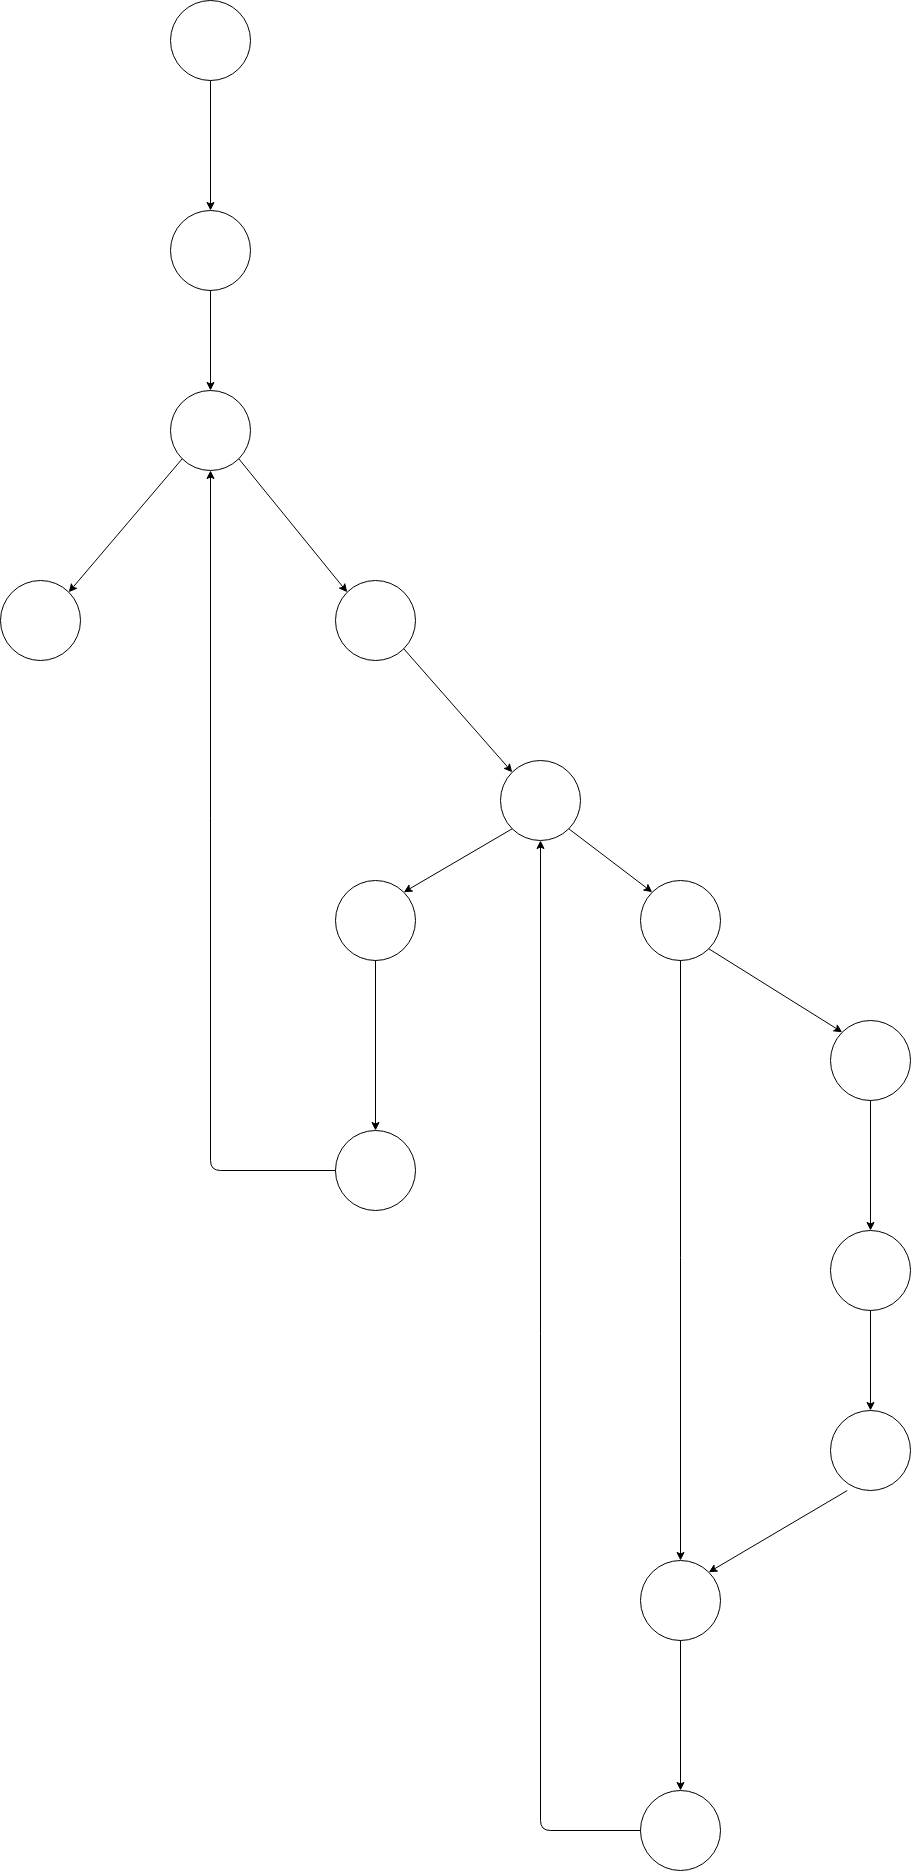
\includegraphics[scale=0.25]{./BubbleSortCFG.png}
\end{enumerate}



\end{document}
